\documentclass{ximera}
\title{How To ...}
\begin{document}

\maketitle
Before you start, here are some directions on how to answer the questions in this test. 
Try this first problem. First try a wrong answer. Also try the hints (there are three levels of them). 
\begin{question}
\begin{solution}
\begin{hint}
$3 \times 2$ is the number of objects in $3$ groups of $2$ objects
\end{hint}
\begin{hint}
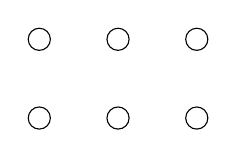
\begin{tikzpicture}
\draw (0,0) circle (4pt);
\draw (1,0) circle (4pt);
\draw (2,0) circle (4pt);
\draw (0,1) circle (4pt);
\draw (1,1) circle (4pt);
\draw (2,1) circle (4pt);
\end{tikzpicture}
\end{hint}
\begin{hint}
$3\times 2=6$
\end{hint}
$3\times 2 = $ \answer{6}
\end{solution}
\end{question}

Sometimes you need to enter an expression as an answer. 
\begin{question}
\textbf{An expression answer type}
\begin{solution}
\begin{hint}
To put $x^2$ you should enter $x$ ^ $2$.
\end{hint}
Try writing the expression $x^2+y$ = \answer{x^2+y}. Remember to try failing as well, to see what happens.
\end{solution}
\end{question}

\begin{question}
\textbf{A matrix answer type}
\begin{solution}
\begin{hint}
See what happens when you click on $+$ and $-$ buttons.
\end{hint}
Try inputing the matrix $\begin{bmatrix} 0&1\\2&3\\0&0\end{bmatrix}$ here
\begin{matrix-answer}[name=M]
correctMatrix = [['0','1'],['2','3'],['0','0']]
\end{matrix-answer}
\end{solution}
\end{question}

\end{document}